% Created 2019-11-12 mar 23:36
\documentclass[presentation,aspectratio=169]{beamer}
\usepackage[utf8]{inputenc}
\usepackage[T1]{fontenc}
\usepackage{fixltx2e}
\usepackage{graphicx}
\usepackage{longtable}
\usepackage{float}
\usepackage{wrapfig}
\usepackage{rotating}
\usepackage[normalem]{ulem}
\usepackage{amsmath}
\usepackage{textcomp}
\usepackage{marvosym}
\usepackage{wasysym}
\usepackage{amssymb}
\usepackage{hyperref}
\tolerance=1000
\usepackage{khpreamble}
\usepackage{xcolor}
\newcommand{\sign}{\mathrm{sign}}
\renewcommand{\transp}{^{\mathrm{T}}}
\usetheme{default}
\author{Kjartan Halvorsen}
\date{2019-11-13}
\title{Robust Kalman filter}
\hypersetup{
  pdfkeywords={},
  pdfsubject={},
  pdfcreator={Emacs 25.3.50.2 (Org mode 8.2.10)}}
\begin{document}

\maketitle
\section{Introduction}
\label{sec-1}
\begin{frame}[label=sec-1-1]{Why a robust version of the Kalman filter?}
\end{frame}
\begin{frame}[label=sec-1-2]{Why a robust version of the Kalman filter?}
The Kalman filter assumes Gaussian measurement noise and so it is very sensitive to outliers. 
\end{frame}
\begin{frame}[label=sec-1-3]{Example 1}
\begin{columns}
\begin{column}{0.3\textwidth}
The target moves in a circle. Observations are noisy with one outlier
\end{column}
\begin{column}{0.7\textwidth}
\begin{center}
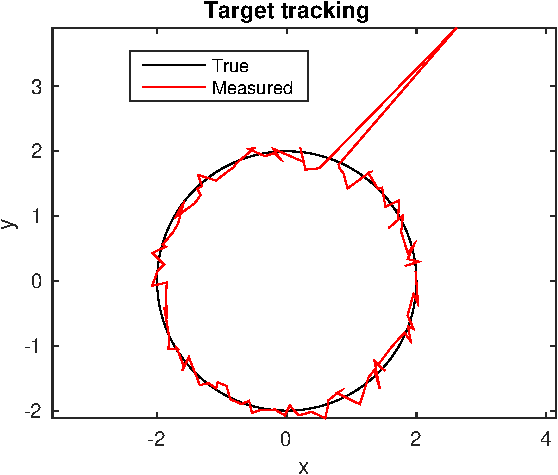
\includegraphics[width=0.9\linewidth]{circular-movement-crop}
\end{center}
\end{column}
\end{columns}
\end{frame}
\begin{frame}[label=sec-1-4]{Example 1 contd.}
The model of the dynamics: \emph{Nearly constant velocity model}
\begin{equation*}
x(k+1) = \bbm I & hI\\ 0 & I \ebm x(k) + \bbm \frac{h^2}{2} I\\hI\ebm v(k),
\end{equation*}
where the state vector contains the position and velocity of the target
\[ x = \bbm p\\\dot{p} \ebm.\]
\end{frame}
\begin{frame}[label=sec-1-5]{Example 1 contd.}
\begin{columns}
\begin{column}{0.3\textwidth}
Result of tracking using standard Kalman filter
\end{column}
\begin{column}{0.7\textwidth}
\begin{center}
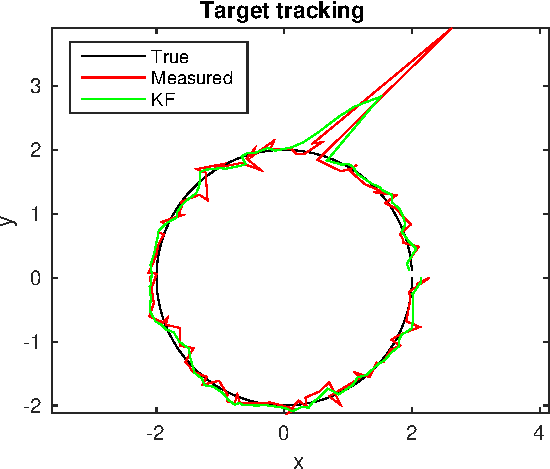
\includegraphics[width=0.9\linewidth]{circular-movement-kf-crop}
\end{center}
\end{column}
\end{columns}
\end{frame}
\section{Convex optimization}
\label{sec-2}
\begin{frame}[label=sec-2-1]{Convex optimization}
\begin{center}

\includegraphics[width=0.7\linewidth]{cvx-book.png}
\end{center}
\end{frame}

\begin{frame}[label=sec-2-2]{Preparation example}
\begin{columns}
\begin{column}{0.4\textwidth}
Linear regression model
\begin{equation*}
y(k) = ax(k) + b + e(k) + w(k), 
\end{equation*}
where $e(k)$ is Gaussian noise and $w(k)$ is a sparse vector of outliers.
\end{column}
\begin{column}{0.6\textwidth}
\begin{center}
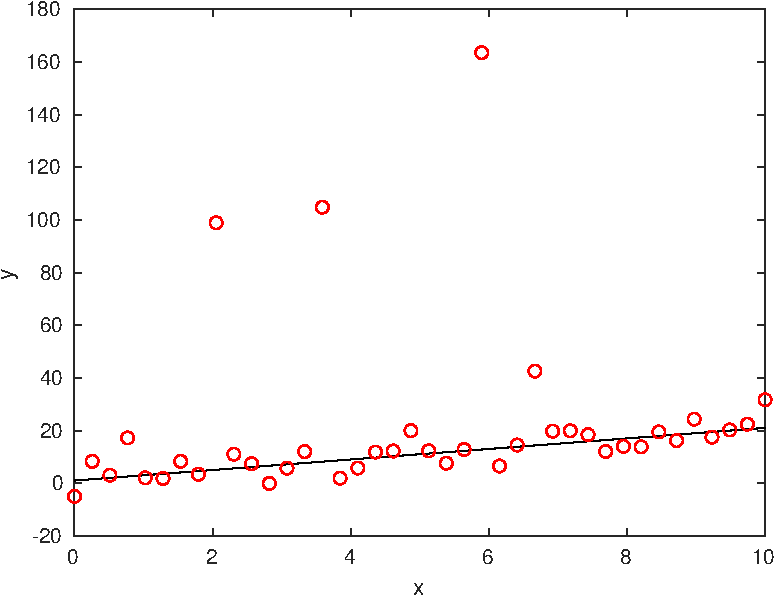
\includegraphics[width=\linewidth]{least_squares_example}
\end{center}
\end{column}
\end{columns}
\end{frame}

\begin{frame}[label=sec-2-3]{Preparation example, contd}
Least squares estimation:
\begin{equation*}
 \text{minimize} \; ||y - ax - b||_2\\
\end{equation*}
Or, equivalently
\begin{align*}
 \text{minimize} \; & ||\epsilon||_2\\
 \text{subject to} \; & \epsilon = y - ax-b
\end{align*}
\end{frame}

\begin{frame}[label=sec-2-4]{Preparation example, contd}
Least squares estimation:
\begin{equation*}
 \text{minimize} \; ||y - ax - b||_2\\
\end{equation*}
Solved by forming 
\[ A = \bbm x(1) & 1\\x(2) & 1\\ \vdots & \vdots\\ x(N) & 1\ebm \]
and
\[ z = \bbm a\\b\ebm, \]
and solving for $z$ in the (over-determined) system of equations
\[ Az = y. \]
\end{frame}

\begin{frame}[label=sec-2-5]{Preparation example, contd}
\begin{columns}
\begin{column}{0.4\textwidth}
\begin{equation*}
 \text{minimize} \; ||y - ax - b||_2\\
\end{equation*}
\end{column}
\begin{column}{0.6\textwidth}
\begin{center}
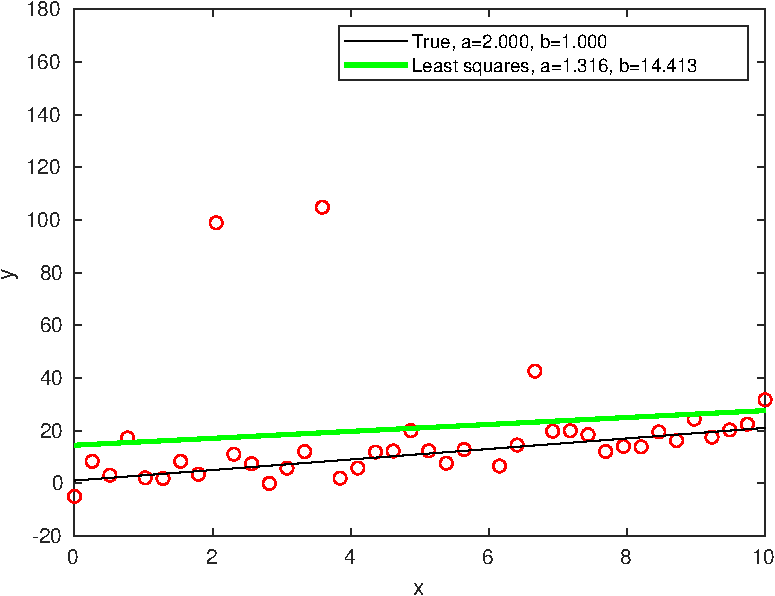
\includegraphics[width=\linewidth]{least_squares_regression}
\end{center}
\end{column}
\end{columns}
\end{frame}

\begin{frame}[label=sec-2-6]{The problem with least squares}
\begin{columns}
\begin{column}{0.4\textwidth}
\begin{align*}
 \text{minimize} \; &\sum_k \phi_{S}(\epsilon_k)\\
 \text{where} \; \phi_S(u) &= u^2
\end{align*}
\end{column}

\begin{column}{0.6\textwidth}

\begin{center}
  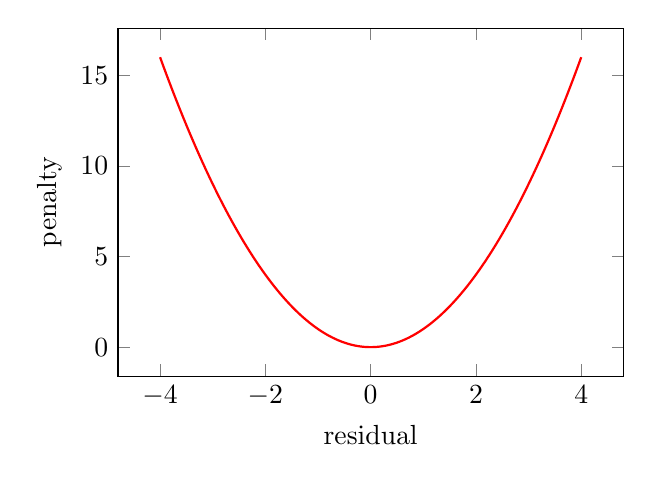
\begin{tikzpicture}
    \begin{axis}[
      width=8cm,
      height=6cm,
      ylabel=penalty,
      xlabel=residual,
      ]
      \addplot[red, thick, no marks, domain=-4:4, samples=201] {x^2};
    \end{axis}
  \end{tikzpicture}
\end{center}
\end{column}
\end{columns}
\end{frame}

\begin{frame}[label=sec-2-7]{More robust: The Huber penalty function}
\begin{columns}
\begin{column}{0.4\textwidth}
Also known as \alert{robust least squares}
\begin{align*}
 \text{minimize} \; &\sum_k \phi_{hub}(\epsilon_k)\\
 \text{where}\; \phi_{hub}(u) &= \begin{cases} u^2 & |u| \le M\\ M(2|u|-M) & |u| > M \end{cases}
\end{align*}
\end{column}

\begin{column}{0.6\textwidth}
\begin{center}
  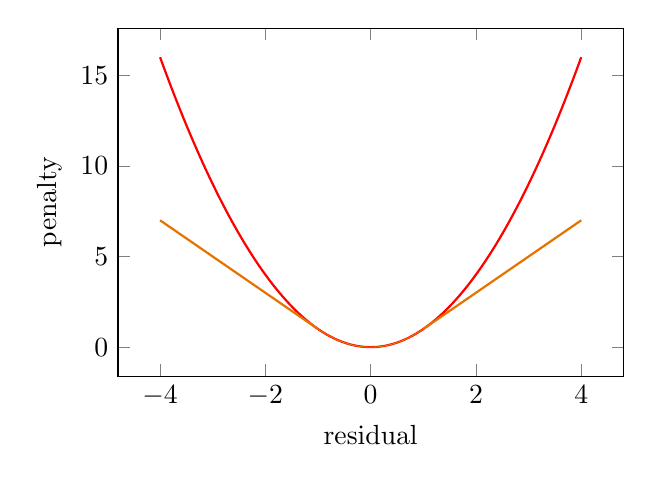
\begin{tikzpicture}
    \begin{axis}[
      width=8cm,
      height=6cm,
      ylabel=penalty,
      xlabel=residual,
      ]
      \addplot[red, thick, no marks, domain=-4:4, samples=201] {x^2};
      \addplot[orange!90!black, thick, no marks, domain=-4:-1, samples=201] {2*abs(x)-1};
      \addplot[orange!90!black, thin, no marks, domain=-1:1, samples=201] {x^2};
      \addplot[orange!90!black, thick, no marks, domain=1:4, samples=201] {2*abs(x)-1};
    \end{axis}
  \end{tikzpicture}
\end{center}
\end{column}
\end{columns}
\end{frame}
\begin{frame}[label=sec-2-8]{Preparation example: Robust least squares}
\begin{columns}
\begin{column}{0.4\textwidth}
\begin{equation*}
 \text{minimize} \; &\sum_k \phi_{hub}(\epsilon_k)\\
\end{equation*}
\end{column}
\begin{column}{0.6\textwidth}
\begin{center}
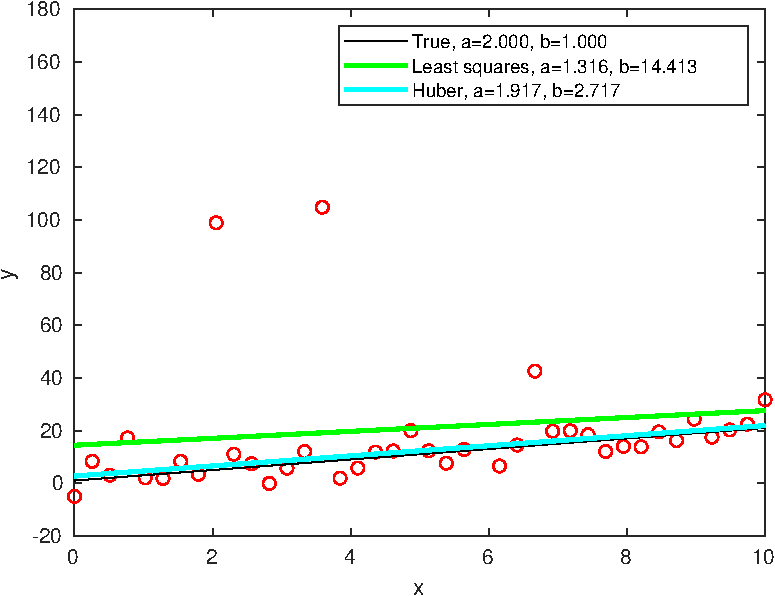
\includegraphics[width=\linewidth]{robust_least_squares_regression}
\end{center}
\end{column}
\end{columns}
\end{frame}



\section{Robust Kalman Filter}
\label{sec-3}
\begin{frame}[label=sec-3-1]{Robustifying the Kalman filter}
\end{frame}
\begin{frame}[label=sec-3-2]{The measurement update of the Kalman filter}
We have the state space model
\begin{align*}
x(k+1) &= Fx(k) + v(k)\\
y(k) &= Hx(k) + e(k) + z(k)\\
e &\sim \mathcal{N}(0,R)\\
v &\sim \mathcal{N}(0,Q)
\end{align*}
The measurement update of the Kalman filter can be shown to be equivalent to solving the problem
\[ \text{minimize} \; (y-Hx)^{\mathrm{T}} R^{-1}(y-Hx) + (x-\hat{x}_{k|k-1})\transp P_{k|k-1}^{-1}(x-\hat{x}_{k|k-1}) \]
The optimal solution is \( x^*=\hat{x}_{k|k} = \hat{x}_{k|k} + K(y-H\hat{x}_{k|k-a}),\) where $K$ is the Kalman gain.
\end{frame}
\begin{frame}[label=sec-3-3]{The measurement update of the Kalman filter}
Introduce $\tilde{x} = x - \hat{x}_{k|k-1}$ and $\tilde{y} = y - H\hat{x}_{k|k-1}$. 
The minimization problem can then be written
\begin{align*}
\text{minimize} \quad  &(y-Hx)^{\mathrm{T}} R^{-1}(y-Hx) + (x-\hat{x}_{k|k-1})\transp P_{k|k-1}^{-1}(x-\hat{x}_{k|k-1})\\
  & \quad = (\tilde{y} -H\tilde{x})\transp R^{-1}(\tilde{y}-H\tilde{x}) + \tilde{x}\transp P_{k|k-1}^{-1}\tilde{x}
 \end{align*}
\end{frame}
\begin{frame}[label=sec-3-4]{The measurement update of the Kalman filter}
We now define the residuals $\epsilon$ for the system of equations
\[ \begin{bmatrix} Z_R & 0\\0 & Z_P \end{bmatrix} \begin{bmatrix}(\tilde{y}-H\tilde{x})\\ \tilde{x} \end{bmatrix} = \epsilon,\]
where $Z_R\transp Z_R = R^{-1}$ and $Z_P\transp Z_P = P_{k|k-1}^{-1}$. 

The minimization problem can now be written
\begin{align*}
\text{minimize} \quad  & \epsilon\transp\epsilon \\
\text{subject to} \quad & \begin{bmatrix} Z_R & 0\\0 & Z_P \end{bmatrix} \begin{bmatrix}(\tilde{y}-H\tilde{x})\\ \tilde{x} \end{bmatrix} = \epsilon,
 \end{align*}
which is a least-squares problem.
\end{frame}
\begin{frame}[label=sec-3-5]{Robustifying the measurement update}
The idea is to use the Huber penalty function $\phi_{hub}$ instead of the quadratic criterion $\epsilon\transp \epsilon$.
\begin{align*}
 \text{minimize} \quad & \sum_{i=1}^{n+m} \phi_{hub}\big( \epsilon(i)\big) \\
\text{subject to} \quad & \begin{bmatrix} Z_R & 0\\0 & Z_P \end{bmatrix} \begin{bmatrix}(\tilde{y}-H\tilde{x})\\ \tilde{x} \end{bmatrix} = \epsilon,
 \end{align*}
\end{frame}


\begin{frame}[label=sec-3-6]{Tracking example again}
\begin{columns}
\begin{column}{0.3\textwidth}
10\% chance of outlier with 10 times normal standard deviation
\end{column}

\begin{column}{0.7\textwidth}
\begin{center}
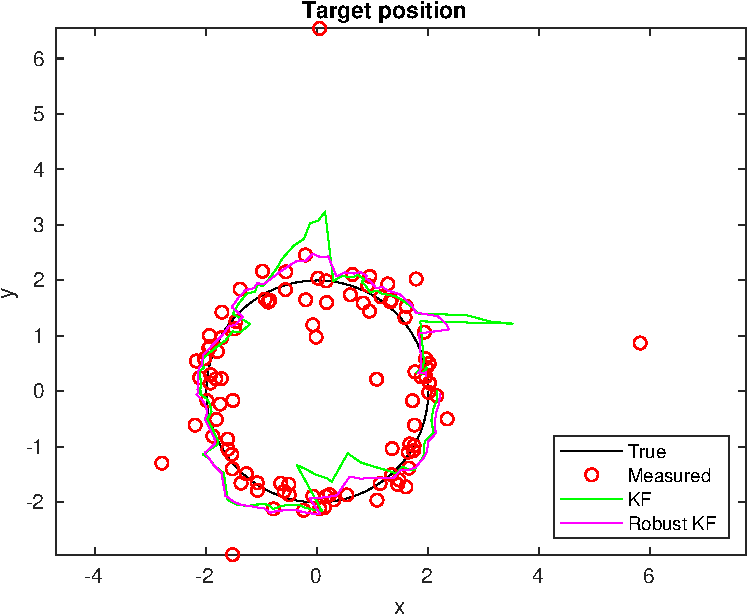
\includegraphics[width=0.9\linewidth]{circular_movement_rkf}
\end{center}
\end{column}
\end{columns}
\end{frame}
% Emacs 25.3.50.2 (Org mode 8.2.10)
\end{document}